We begin with a negative result: in the worst case, there may not be an exact proportional solution. The impossibility remains even in the special case when $\N = \M$. The latter construction is slightly more involved; we begin with the arbitrary $\N$ and $\M$ setting. The basic idea behind both constructions is to create two groups of points very far away from one another with $k=3$, ensuring that one group will be served by only one center. 

\begin{claim}
\label{claim:lowerBound}
	For all $\rho < 2$, a $\rho$-proportional solution is not guaranteed to exist.
\end{claim}
\begin{proof}
	Consider the following instance with $\N = \{a_1,  a_2, \hdots, a_6\}$, $\M = \{x_1, x_2, \hdots, x_6\}$ and $k=3$. Distances are specified in the following table.
\begin{center}
  \begin{tabular}{|c || c | c | c | c | c | c  |} 
  \hline 
         & $x_1$   & $x_2$  & $x_3$    & $x_4$  & $x_5$   & $x_6$   \\ \hline \hline
  $a_1$ &  4     & 1 & 2    & $\infty$ & $\infty$ & $\infty$  \\ \hline
  $a_2$ & 2    &   4    & 1  & $\infty$ & $\infty$ & $\infty$  \\ \hline  
  $a_3$ & 1  &  2  &   4     & $\infty$ & $\infty$ & $\infty$  \\ \hline
  $a_4$ & $\infty$ & $\infty$ & $\infty$ &    4    & 1 &  2    \\ \hline
  $a_5$ & $\infty$ & $\infty$ & $\infty$ &   2  &    4   & 1   \\ \hline
  $a_6$ & $\infty$ & $\infty$ & $\infty$ & 1  &  2  &   4       \\ \hline
\end{tabular}
\end{center}

Notice that the data is separate into two areas. Since $k=3$, in a feasible solution, we only open one center in one of these two areas. Without loss of generality, suppose that we open exactly one center among $\{x_1, x_2, x_3\}$. The instance is symmetric, so again suppose without loss of generality that we open $x_1$. Then consider the individuals in $\{a_1, a_2\}$. This coalition is of size $\lceil \frac{n}{k} \rceil = 2$, and both individuals would reduce their distance by a factor of $2$ by switching to $x_3$. Thus, any solution is only 2-proportional. 
\end{proof}

\begin{claim}
	In the special case where $\N = \M$, for all $\rho < 1.5$, a $\rho$-proportional solution is not guaranteed to exist.
\end{claim}
\begin{proof}
	Let $k=5$. There are three identical clusters of 303 points each (so $n = 909$). The pairwise distance between any two points in different clusters is $\infty$. Construct each cluster as follows. There are six types of points, $a_1, a_2, a_3, x_1, x_2, x_3$ (all feasible, since $\M = \N$). There is exactly one point of type $x_1$, one point of type $x_2$, and one point of type $x_3$. There are 100 points each of type $a_1$, $a_2$, and $a_3$ (that is, there are 100 points co-located at each position). The pairwise distance between points in a cluster of given types is specified in the following table. The pairwise distance between any two points of types in $\{x_1, x_2, x_3\}$ is equal to the distance between any two points of types in $\{a_1, a_2, a_3\}$ is equal to 3, which follows from the shortest path distances on a weighted bipartite graph with weights defined by the table. 
		
\begin{center}
  \begin{tabular}{|c || c | c | c |} 
  \hline 
         & $x_1$ & $x_2$ & $x_3$ \\ \hline \hline
  $a_1$ & 4     &  1        & 2         \\ \hline
  $a_2$ & 2     &  4        & 1         \\ \hline  
  $a_3$ & 1     &  2        & 4         \\ \hline
\end{tabular}
\end{center}

Since $k = 5$ and there are three clusters, in a feasible solution there is a cluster in which we choose at most one center. In that cluster, suppose first that we choose a center of type $x_1$, $x_2$, or $x_3$. Since the instance is symmetric with respect to this choice, suppose without loss of generality that we choose $x_1$. Then the 200 points of types $a_1$ and $a_2$ could decrease their distance by a factor of $2$ by switching to $x_3$. Since any $\lceil 909/5 \rceil = 182$ points are entitled to deviate, such a choice of $x_1$ is not $\rho$-proportional for $\rho < 2$. 

Instead, suppose that we choose a center of type $a_1$, $a_2$, or $a_3$. The instance is again symmetric with respect to this choice, so suppose without loss of generality that we choose $a_1$. Then the 200 points of types $a_2$ and $a_3$ could decrease their distance by a factor of 1.5 by switching to $x_1$. Thus, in either case, the solution is not $\rho$-proportional for any $\rho < 1.5$. 
\end{proof}

\subsection{Computing a $ \left(1+\sqrt{2} \right)$-Approximate Proportional Clustering}
Claim~\ref{claim:lowerBound} establishes that we should focus our attention on designing an efficient approximation algorithm. We give a simple and efficient algorithm that achieves a $\left( 1 + \sqrt{2} \right)$-proportional solution, very close to the existential lower bound of 2. For notational ease, let $B(x, \delta) = \{i \in \N: \; d(i, x) \leq \delta\}$. That is, $B(x, \delta)$ is the ball (defined on $\N$) of distance $\delta$ about center $x$. For simplicity of exposition, we present Algorithm~\ref{alg:ball} as a \textit{continuous} algorithm where a $\delta$ parameter is smoothly increasing. The algorithm can be easily discretized using priority queues. 

\begin{algorithm}
\begin{algorithmic}[1]
\caption{Greedy Capture}
\label{alg:ball}
	\STATE $\delta \gets 0$; $X \gets \emptyset$; $N \gets \N$
	\WHILE{$N \neq \emptyset$}
		\STATE Smoothly increase $\delta$
		\WHILE{$\exists x \in X$ s.t. $|B(x, \delta) \cap N| \geq 1$}
			\STATE $N \gets N \backslash B(x, \delta)$
		\ENDWHILE
		\WHILE{$\exists x \in ( \M \backslash X)$ s.t. $|B(x, \delta) \cap N| \geq \lceil \frac{n}{k} \rceil$}
			\STATE $X \gets X \cup \{x\}$
			\STATE $N \gets N \backslash B(x, \delta)$
		\ENDWHILE
	\ENDWHILE
	\STATE return X
\end{algorithmic}
\end{algorithm}

Algorithm~\ref{alg:ball} runs in $\tilde{O}(mn)$ time.\footnote{To state running times simply, we use the convention that $f(n)$ is $\tilde{O}(g(n))$ if $f(n)$ is $O(g(n))$ up to poly-logarithmic factors.} In essence, the algorithm grows balls continuously around the centers, and when the ball around a center has ``captured'' $\lceil \frac{n}{k} \rceil$ points, we greedily open that center and disregard all of the captured points. Open centers continue to greedily capture points as their balls continue to expand. Though~\cite{kMedianPrimalDual,mettuPlaxton} similarly expand balls about points to compute approximately optimal solutions to the $k$-median problem, there is a crucial difference: They grow balls around data points rather than centers. %in a succession of subsamples aimed at minimizing the objective value, rather than a single greedy process.

\begin{theorem}
\label{thm:ballGrowing}
	Algorithm~\ref{alg:ball} yields a $(1+\sqrt{2})$-proportional clustering, and there exists an instance for which this bound is tight.
\end{theorem}
\begin{proof}
	Let $X$ be the solution computed by Algorithm~\ref{alg:ball}. First note that $X$ uses at most $k$ centers, since it only opens a center when $\lceil \frac{n}{k} \rceil$ \textit{unmatched} points are absorbed by the ball around that center, and this can happen at most $k$ times. Now, suppose for a contradiction that $X$ is not a $(1+\sqrt{2})$-proportional clustering. Then there exists $S \subseteq \N$ with $|S| \geq \lceil \frac{n}{k} \rceil$ and $y \in \M$ such that \begin{equation} \label{eq:contradiction} \forall i \in S, \; (1+\sqrt{2}) \cdot d(i, y) < D_i(X).\end{equation} 

Let $r_y$ be the distance of the farthest agent from $y$ in $S$, that is, $r_y := \max_{i \in S} d(i, y)$, and call this agent $i^*$. There are two cases. In the first case, $B(x, r_y) \cap S = \emptyset$ for all $x \in X$. This immediately yields a contradiction, because it implies that Algorithm 1 would have opened $y$. In particular, note that $S \subseteq B(y, r_y)$, so if $S \cap B(x, r_y) = \emptyset$ for all $x \in X$, then $B(y, r_y)$ would have had at least $\lceil \frac{n}{k} \rceil$ unmatched points.

\begin{figure}[!h]
\centering
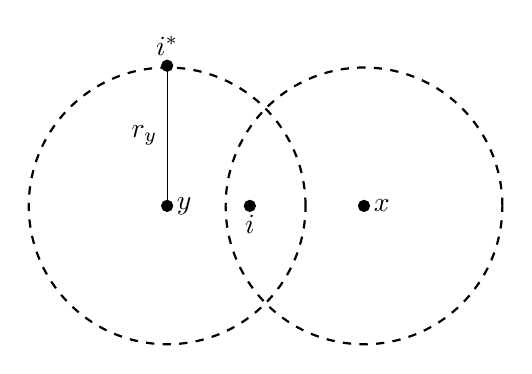
\begin{tikzpicture}
	\filldraw[black] (-1.25,0) circle (2pt) node[anchor=west] {$y$};
	\draw[black, thick, dashed] (-1.25,0) circle (50pt);
	
	\filldraw[black] (1.25,0) circle (2pt) node[anchor=west] {$x$};
	\draw[black, thick, dashed] (1.25,0) circle (50pt);
	
	\filldraw[black] (-1.25,1.78) circle (2pt) node[anchor=south] {$i^*$};
	\draw (-1.25,0) -- (-1.25, 1.78);
	\filldraw[black] (-1.25,0.89) circle (0pt) node[anchor=east] {$r_y$};
	
	\filldraw[black] (-0.2,0) circle (2pt) node[anchor=north] {$i$};
	
	\end{tikzpicture}
\caption{Diagram for Proof of Theorem~\ref{thm:ballGrowing}}
\label{fig:ballProof}
\end{figure}

In the second case, $\exists x \in X$ and $\exists i \in N$ such that $i \in B(x, r_y) \cap S$. This case is drawn below in Figure~\ref{fig:ballProof}. By the triangle inequality, $d(x, y) \leq d(i, x) + d(i, y)$. Therefore, $d(i^*, x) \leq r_y + d(i, x) + d(i, y)$. Also, $d(i, x) \leq r_y$, since $i \in B(x, r_y)$. Consider the minimum multiplicative improvement of $i$ and $i^*$: 

 
\begin{equation*}
\begin{split}
	&\min\left( \frac{d(i, x)}{d(i, y)}, \; \frac{d(i^*, x)}{d(i^*, y)} \right) \\
	& \leq \min\left( \frac{d(i, x)}{d(i, y)}, \; \frac{r_y + d(i, x) + d(i, y)}{r_y} \right) \\
	& \leq \min\left( \frac{r_y}{d(i, y)}, \; 2 + \frac{d(i, y)}{r_y} \right) \\
	& \leq \max_{z \geq 0} \left( \min \left( z,\; 2+1/z\right) \right) = 1 + \sqrt{2} 
\end{split}
\end{equation*}
which violates equation~\ref{eq:contradiction}. 

It is not hard to show that there exists an instance for which Algorithm~\ref{alg:ball} yields exactly this bound. Consider the following instance with $\N = \{a_1,  a_2, \hdots, a_6\}$, $\M = \{x_1, x_2, x_3, x_4\}$ and $k=3$. Distances are specified in the following table, where $\epsilon > 0$ is some small constant.
\begin{center}
  \begin{tabular}{|c || c | c | c | c | c | c  |} 
  \hline 
             & $x_1$          & $x_2$       & $x_3$          & $x_4$             \\ \hline \hline
  $a_1$ & 1                  & $1+\sqrt{2}$ & $\infty$        & $\infty$         \\ \hline
  $a_2$ & $\sqrt{2}-1$ &  $1-\epsilon$ & $\infty$        & $\infty$         \\ \hline  
  $a_3$ & $1+\sqrt{2}$ &  $1-\epsilon$ & $\infty$        & $\infty$          \\ \hline
  $a_4$ & $\infty$         & $\infty$     & 1                  &   $1+\sqrt{2}$ \\ \hline
  $a_5$ & $\infty$         & $\infty$     & $\sqrt{2}-1$  &   $1-\epsilon$ \\ \hline
  $a_6$ & $\infty$         & $\infty$     & $1+\sqrt{2}$ & $1-\epsilon$  \\ \hline
\end{tabular}
\end{center}
The distances satisfy the triangle inequality. Note that Algorithm~\ref{alg:ball} will open $x_2$ and $x_4$. The coalition $\{a_1, a_2\}$ can each reduce their distance by a multiplicative factor approaching $1+\sqrt{2}$ as $\epsilon \rightarrow 0$ by deviating to $x_1$.
\end{proof}

\subsection{Local Capture Heuristic}
We observe that while our Greedy Capture algorithm (Algorithm~\ref{alg:ball}) always produces an approximately proportional solution, it may not produce an exactly proportional solution in practice, even on instances where such solutions exist (see Figure~\ref{fig:IrisRho} and Figure~\ref{fig:DiabetesRho}). We therefore introduce a Local Capture heuristic for searching for more proportional clusterings. Algorithm~\ref{alg:local} takes a target value of $\rho$ as a parameter, and proceeds by iteratively finding a center that violates $\rho$-fairness and swapping it for the center in the current solution that is least demanded.

\begin{algorithm}
\begin{algorithmic}[1]
\caption{Local Capture Heuristic}
\label{alg:local}
	\INPUT $\rho$
	\STATE Initialize $X$ as a random subset of $k$ centers from $\M$.
	\REPEAT
	\FOR{$y \in \M$}
		\STATE $S_y \gets \{i \in N: \rho \cdot d_{iy} < D_i(X)\}$
		\IF{$|S_y| \geq \lceil \frac{n}{k} \rceil$} 
			\STATE $x^* \gets \mbox{argmin}_{x \in X} | \{i \in N: d_{ix} = D_i(X) \}|$
			\STATE $X \gets (X \backslash \{x^*\}) \cup \{y\}$
		\ENDIF
	\ENDFOR
	\UNTIL{no changes occur}
	\STATE return X
\end{algorithmic}
\end{algorithm}

Every iteration of Algorithm~\ref{alg:local} (the entire inner for loop) runs in $\tilde{O}(mn^2)$ time. There is no guarantee of convergence (for a given input $\rho$, there may not even exist a $\rho$-proportional solution), but if Algorithm~\ref{alg:local} terminates, then it returns a $\rho$-proportional solution. In our experiments (see Section~\ref{sec:experiments}), we search for the minimum $\rho$ for which the algorithm terminates in a small number of iterations via binary search over possible input of $\rho$. In~\cite{kmedians}, the authors also evaluate a local search swapping procedure for the $k$-median problem, but their swap condition is based on the relative $k$-median objective of two solutions, whereas our swap condition is based on violations to proportionality.